\documentclass[main.tex]{subfiles}
\begin{document}
\begin{bmcsex}{Bond damage and plasticity}{e23_bond_slip_damage_plasticity}
\noindent This example shows the response of bond material point 
which enters simultaneously the yielding and damage regime. Damage is 
increasing during the first loading branch. Subsequently, the exhibits
material point exhibits kinematic hardening upon unloading and reloading.
 \\
\begin{center}
            
{\scriptsize 
\begin{longtable}{lrp{4cm}}\toprule
\textbf{\textsf{Model parameter}} 
& 
\textbf{\textsf{Symbol = Value [Unit]}} 
&
\textbf{\textsf{Description}}  \\\midrule \midrule
\texttt{n\_steps} & $n_\mathrm{s}$ = 100 [-] & {\footnotesize None}  \\
            \texttt{material\_model} & option = damage-plasticity [-] & {\footnotesize None}  \\
            \texttt{interaction\_type} & option = predefined [-] & {\footnotesize None}  \\
            \midrule
\multicolumn{3}{l}{\textbf{\textsf{LoadingScenario: loading\_scenario}}}\\

\texttt{loading\_scenario.number\_of\_cycles} & $n_\mathrm{cycles}$ = 3 [-] & {\footnotesize None}  \\
            \texttt{loading\_scenario.number\_of\_increments} & $n_{\mathrm{incr}}$ = 20 [-] & {\footnotesize None}  \\
            \texttt{loading\_scenario.loading\_type} & option = cyclic [-] & {\footnotesize None}  \\
            \texttt{loading\_scenario.maximum\_loading} & $\phi_{\max}$ = 0.003 [-] & {\footnotesize None}  \\
            \texttt{loading\_scenario.amplitude\_type} & option = constant [-] & {\footnotesize None}  \\
            \texttt{loading\_scenario.unloading\_ratio} & $\phi_{\mathrm{unload}}$ = 0.8 [-] & {\footnotesize None}  \\
            \texttt{loading\_scenario.loading\_range} & option = symmetric [-] & {\footnotesize None}  \\
            
\multicolumn{3}{r}{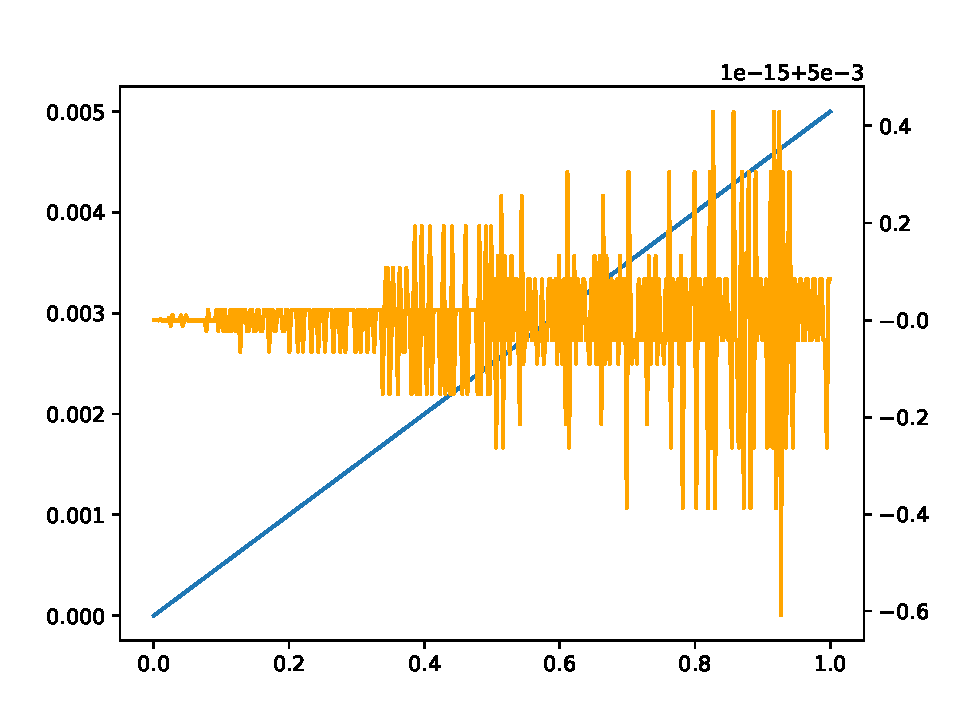
\includegraphics[width=5cm]{examples/e23_bond_slip_damage_plasticity/fig_loading_scenario.pdf}}\\
\midrule
\multicolumn{3}{l}{\textbf{\textsf{MATSBondSlipDP: mats\_eval}}}\\

\texttt{mats\_eval.E\_b} & $E_\mathrm{b}$ = 12900 [MPa/mm] & {\footnotesize Bond stiffness}  \\
            \texttt{mats\_eval.K} & $K$ = 1000.0 [MPa/mm] & {\footnotesize Isotropic hardening modulus}  \\
            \texttt{mats\_eval.tau\_bar} & $\bar{\tau}$ = 5 [MPa] & {\footnotesize Yield stress}  \\
            \texttt{mats\_eval.omega\_fn\_type} & None = li [None] & {\footnotesize None}  \\
            \texttt{mats\_eval.gamma} & $\gamma$ = 0.0 [MPa/mm] & {\footnotesize Kinematic hardening modulus}  \\
            \midrule
\multicolumn{3}{l}{\textbf{\textsf{LiDamageFn: omega\_fn}}}\\

\texttt{mats\_eval.omega\_fn.s\_0} & $s_0$ = 0.0004 [None] & {\footnotesize elastic strain limit}  \\
            \texttt{mats\_eval.omega\_fn.alpha\_2} & $\alpha_2$ = 2000.0 [None] & {\footnotesize parameter controls the damage function}  \\
            \texttt{mats\_eval.omega\_fn.alpha\_1} & $\alpha_1$ = 1.0 [None] & {\footnotesize parameter controls the damage function}  \\
            
\multicolumn{3}{r}{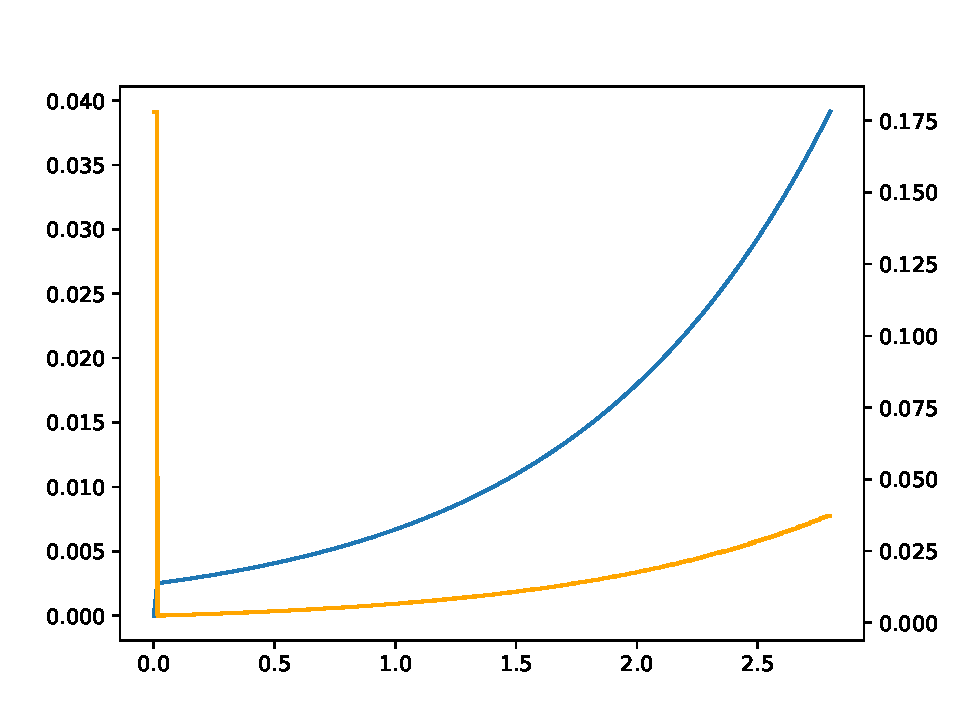
\includegraphics[width=5cm]{examples/e23_bond_slip_damage_plasticity/fig_Li_damage_function.pdf}}\\
\bottomrule 
\end{longtable}
}

\noindent
\begin{longtable}{L{7.5cm}L{7.5cm}}
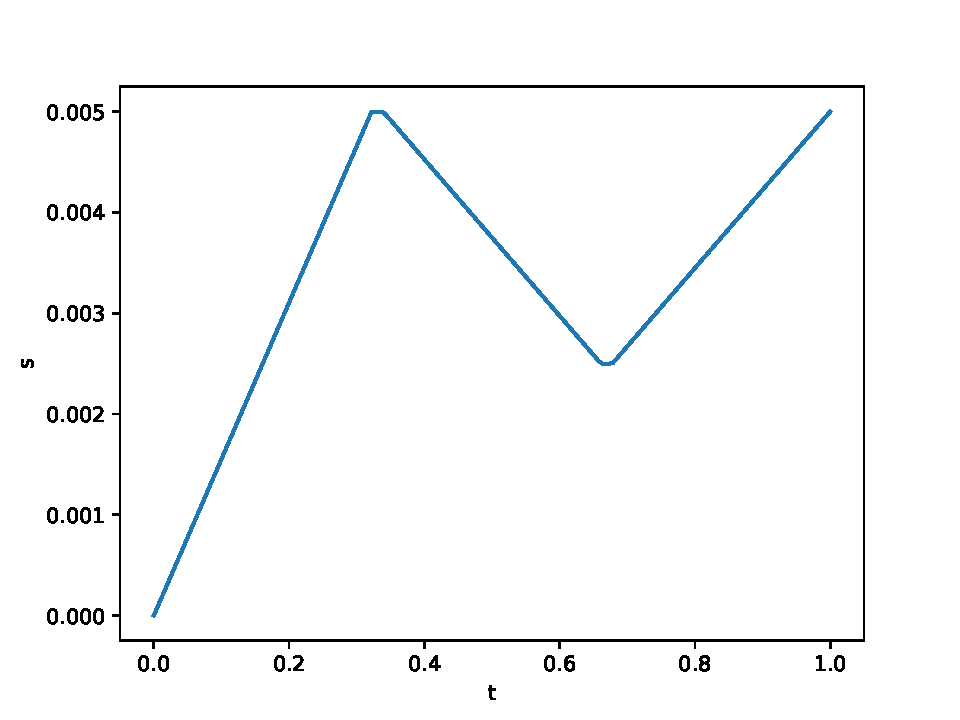
\includegraphics[width=7.5cm]{examples/e23_bond_slip_damage_plasticity/fig_s-t.pdf}
 & 
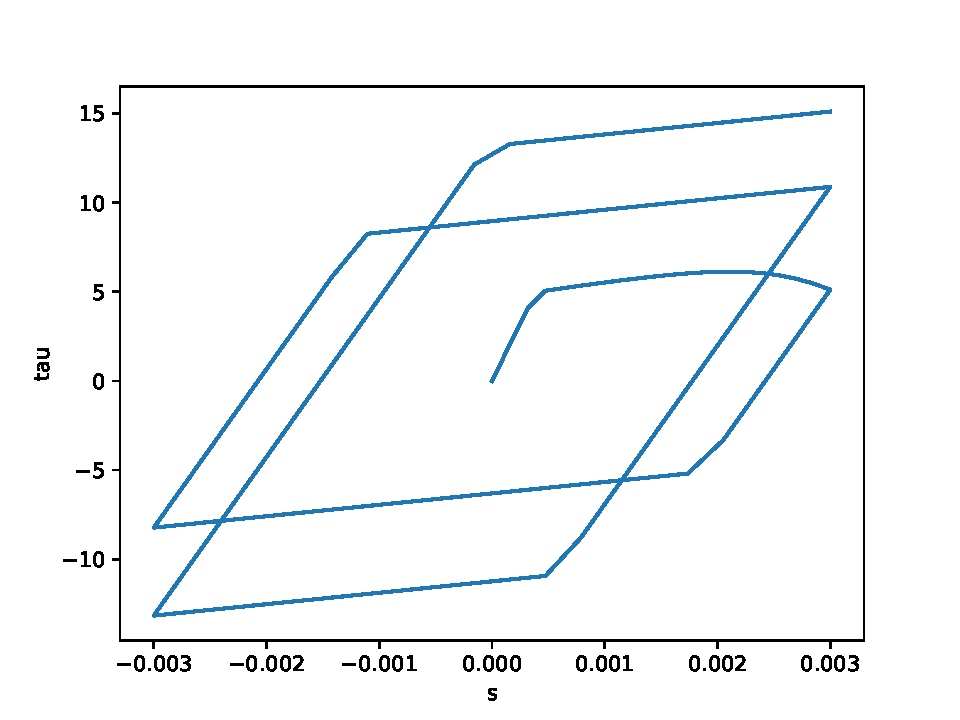
\includegraphics[width=7.5cm]{examples/e23_bond_slip_damage_plasticity/fig_tau-s.pdf}
 \\\end{longtable}

\noindent
\begin{longtable}{L{7.5cm}L{7.5cm}}
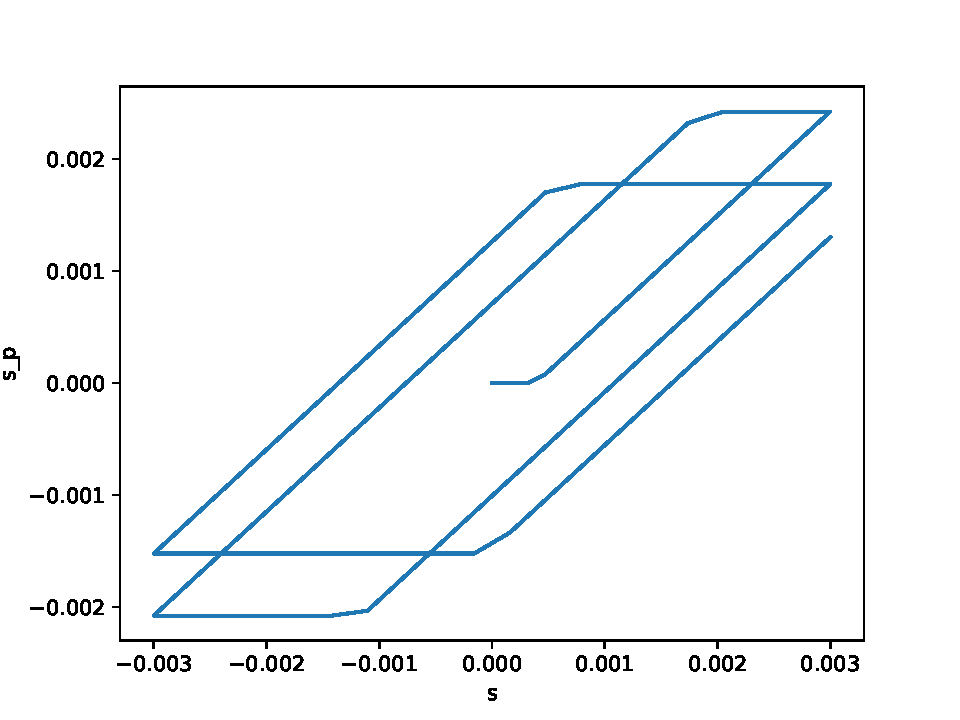
\includegraphics[width=7.5cm]{examples/e23_bond_slip_damage_plasticity/fig_s_p-s.pdf}
 & 
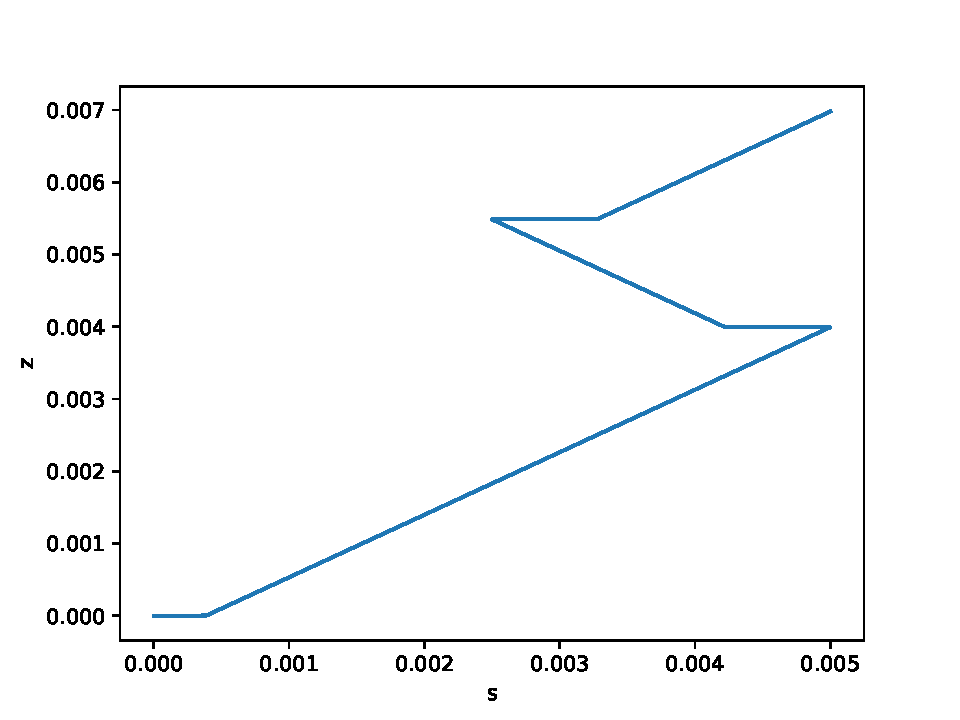
\includegraphics[width=7.5cm]{examples/e23_bond_slip_damage_plasticity/fig_z-s.pdf}
 \\\end{longtable}

\noindent
\begin{longtable}{L{7.5cm}L{7.5cm}}
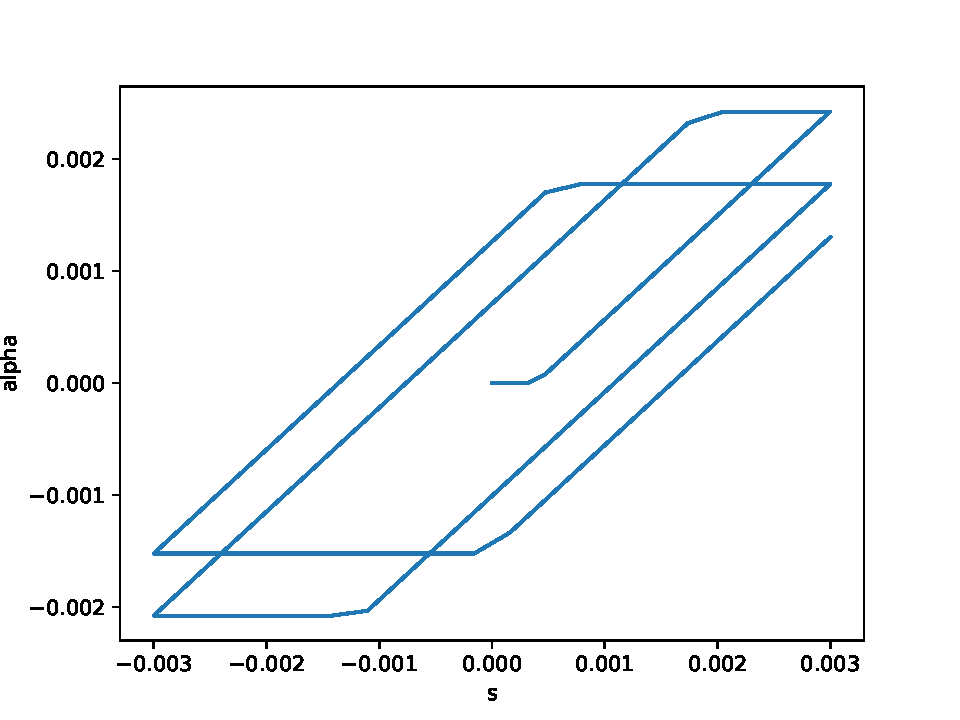
\includegraphics[width=7.5cm]{examples/e23_bond_slip_damage_plasticity/fig_alpha-s.pdf}
 & 
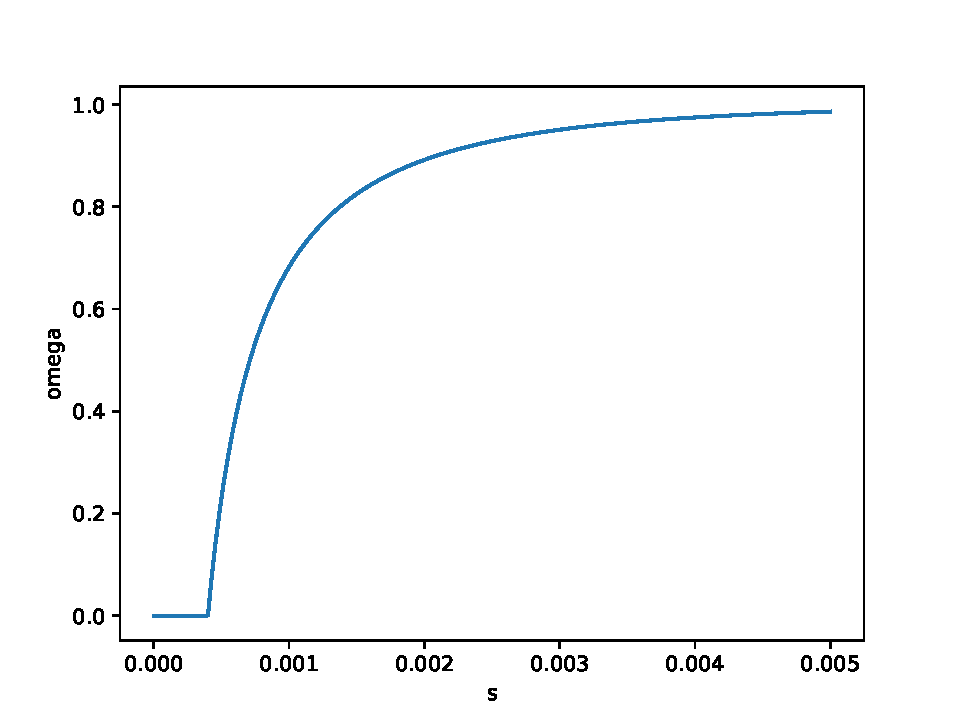
\includegraphics[width=7.5cm]{examples/e23_bond_slip_damage_plasticity/fig_omega-s.pdf}
 \\\end{longtable}
\end{center}
            \end{bmcsex}
\end{document}
    